%----------------------------------------------------------------------
\begin{frame}{A more complicated multistate model}
\vspace*{-1em}
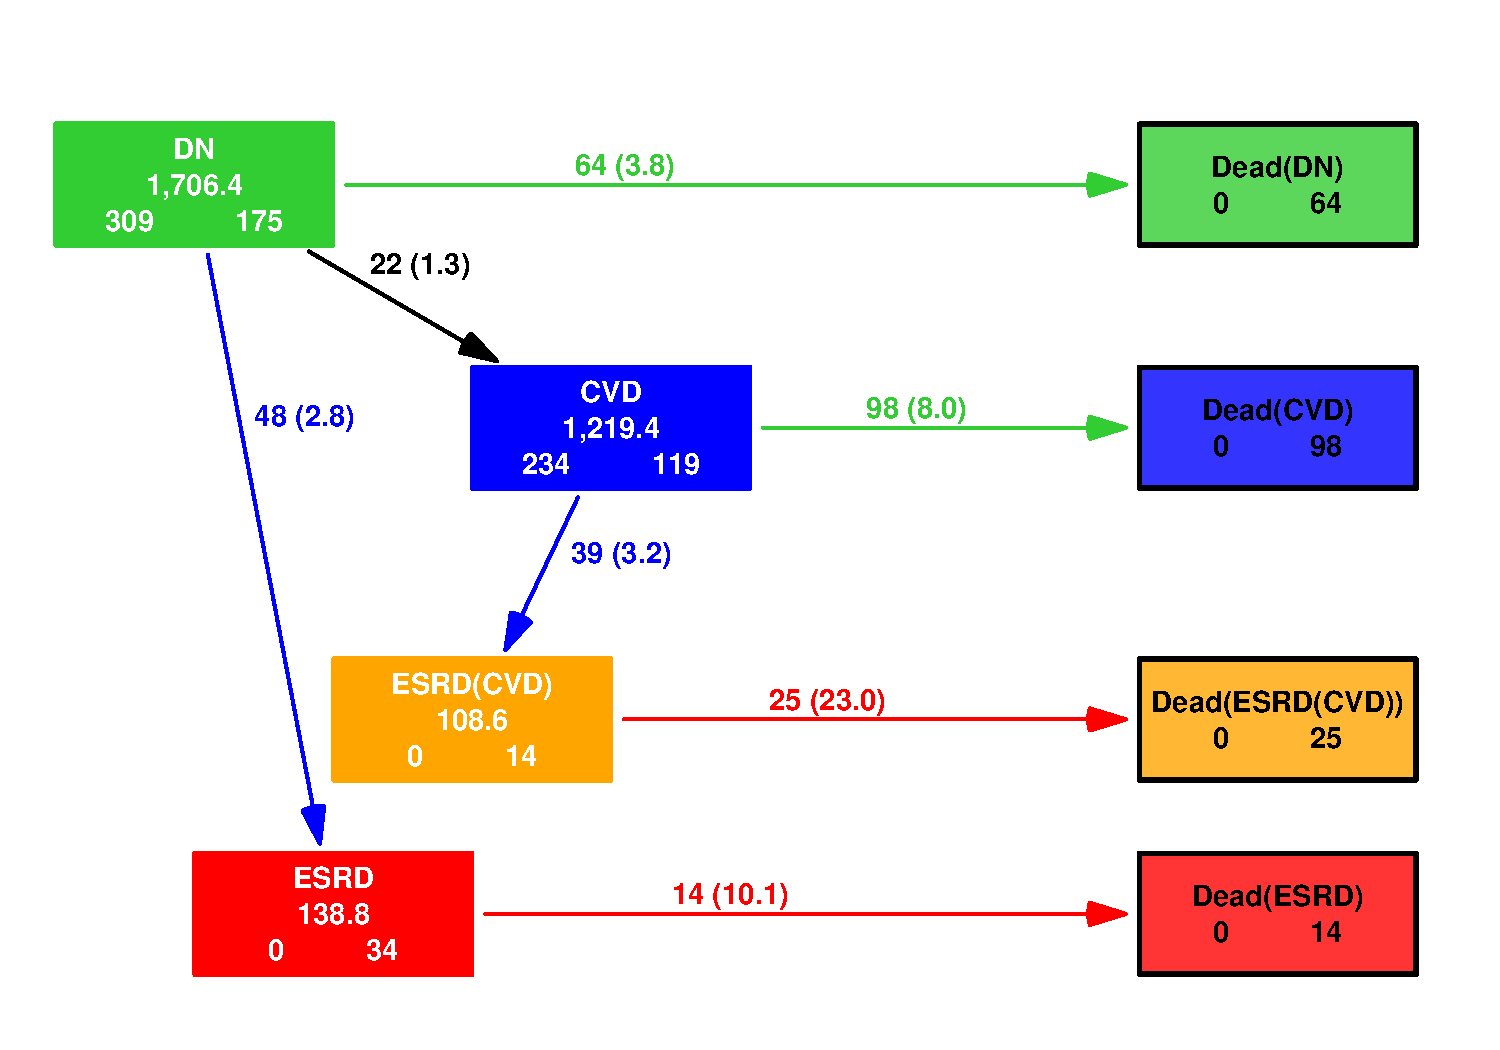
\includegraphics[width=0.82\textwidth]{./GbAd-states.pdf}
\end{frame}

%----------------------------------------------------------------------
\begin{frame}{A more complicated multistate model}
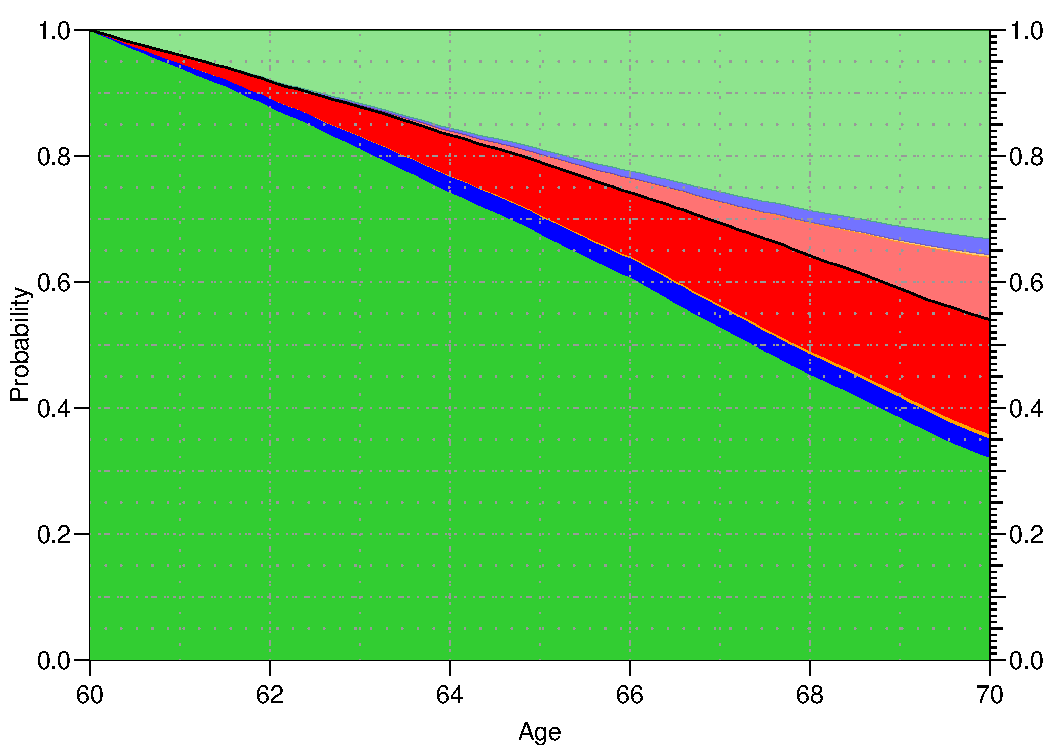
\includegraphics[width=0.75\textwidth]{./GbAd-probs.pdf}
\end{frame}

%----------------------------------------------------------------------
\begin{frame}
   \frametitle{State probabilities}
   How do we get from rates to probabilities:
\pause
   \begin{itemize}[<+->]
   \item 1: Analytical calculations:

 \begin{itemize}[<+->]
     \item immensely complicated formulae
     \item computationally fast (once implemented)
     \item difficult to generalize
     \end{itemize}

   \item 2: Simulation of persons' histories

     \begin{itemize}[<+->]
     \item conceptually simple
     \item computationally not quite simple
     \item easy to generalize
     \item hard to get confidence intervals (bootstrap)
     \end{itemize}

   \end{itemize}
\end{frame}

% %----------------------------------------------------------------------
% \begin{frame}
%    \frametitle{Simulation of a survival time}
%    \begin{itemize}[<+->]
%    \item For a rate function $\lambda(t)$,
%      $\Lambda(t)=\int_0^t\lambda(s) \dif s$:
% \[
%    S(t) = \exp\bigl( -\Lambda(t) \bigr)
% \]
%    \item Simulate a survival probability $u \in [0,1]$:
% \[
%     u = S(t) \quad \Leftrightarrow \quad \Lambda(t) = -\log(u)
% \]
%    \item Knowledge of $\Lambda(t)$ makes it easy to find a survival time\\
%       --- essentially just linear interpolation.
%    \end{itemize}
% \end{frame}

% %----------------------------------------------------------------------
% \begin{frame}[fragile]
%   \frametitle{Simulation of a survival time}
% Simulated random variate: $u$:
% \[
% u=0.853 \quad \Leftrightarrow \quad -\log(u) = 0.159
% \]
% Look up $0.159$ in the
% table of the cumulative rates $\Lambda(t)$:

% \renewcommand{\baselinestretch}{0.8}
% \small
% \begin{semiverbatim}
% time  Lambda
%  ...
%  1.2   0.131
%  1.3   \alert<2->{0.151}
%  1.4   \alert<2->{0.165}
%  1.5   0.181
%  ...
% \end{semiverbatim}
% \normalsize
% \renewcommand{\baselinestretch}{1.0}
% \pause
% \pause
% Linear interpolation gives:
% \[
% t = 1.3 + 0.1 \times (0.159-0.151)/(0.165-0.151) = 1.357
% \]
% \end{frame}

% %----------------------------------------------------------------------
% \begin{frame}
%    \frametitle{Simulation of one survival time}
%    \begin{itemize}[<+->]
%    \item Cumulative rates as a function of time
%    \item Obtained from a model for the mortality rates:

%      \begin{itemize}[<+->]
%      \item Cox-model:\\
%  Cumulative incidence directly --- the Breslow estimator
%      \item Poisson model:\\
%  Estimated incidence rates cumulated
%      \item \ldots
%      \end{itemize}
%    \item Simulate survival probability
%    \item Invert to time by look-up in table
%    \end{itemize}
% \end{frame}

%----------------------------------------------------------------------
\begin{frame}
   \frametitle{Simulation in a multistate model}
\vspace*{-1ex}
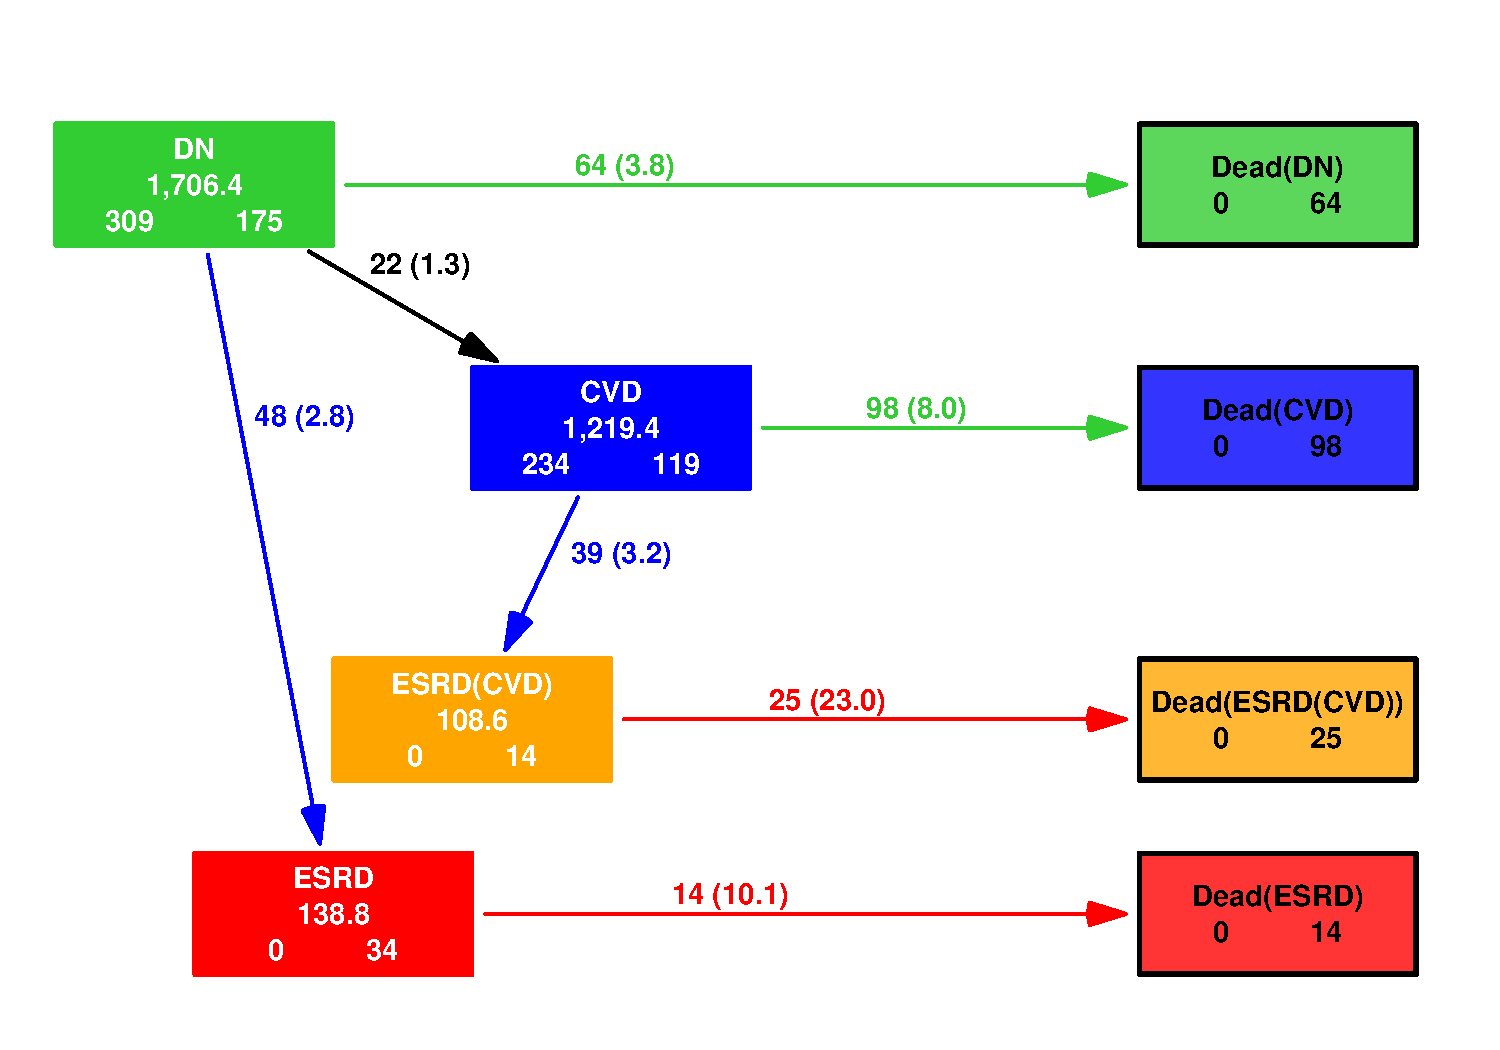
\includegraphics[width=0.45\textwidth]{./GbAd-states.pdf}
\pause
\vspace*{-1ex}
   \begin{itemize}[<+->]
   \item Simulate a ``survival time'' for each transition
     \textbf{out} of a state.
   \item The smallest of these is the transition time.
   \item Choose the corresponding transition type as transition.
   \end{itemize}
\end{frame}

%----------------------------------------------------------------------
\begin{frame}[fragile]
   \frametitle{Transition object are \texttt{glm}s}
\vspace*{-1ex}
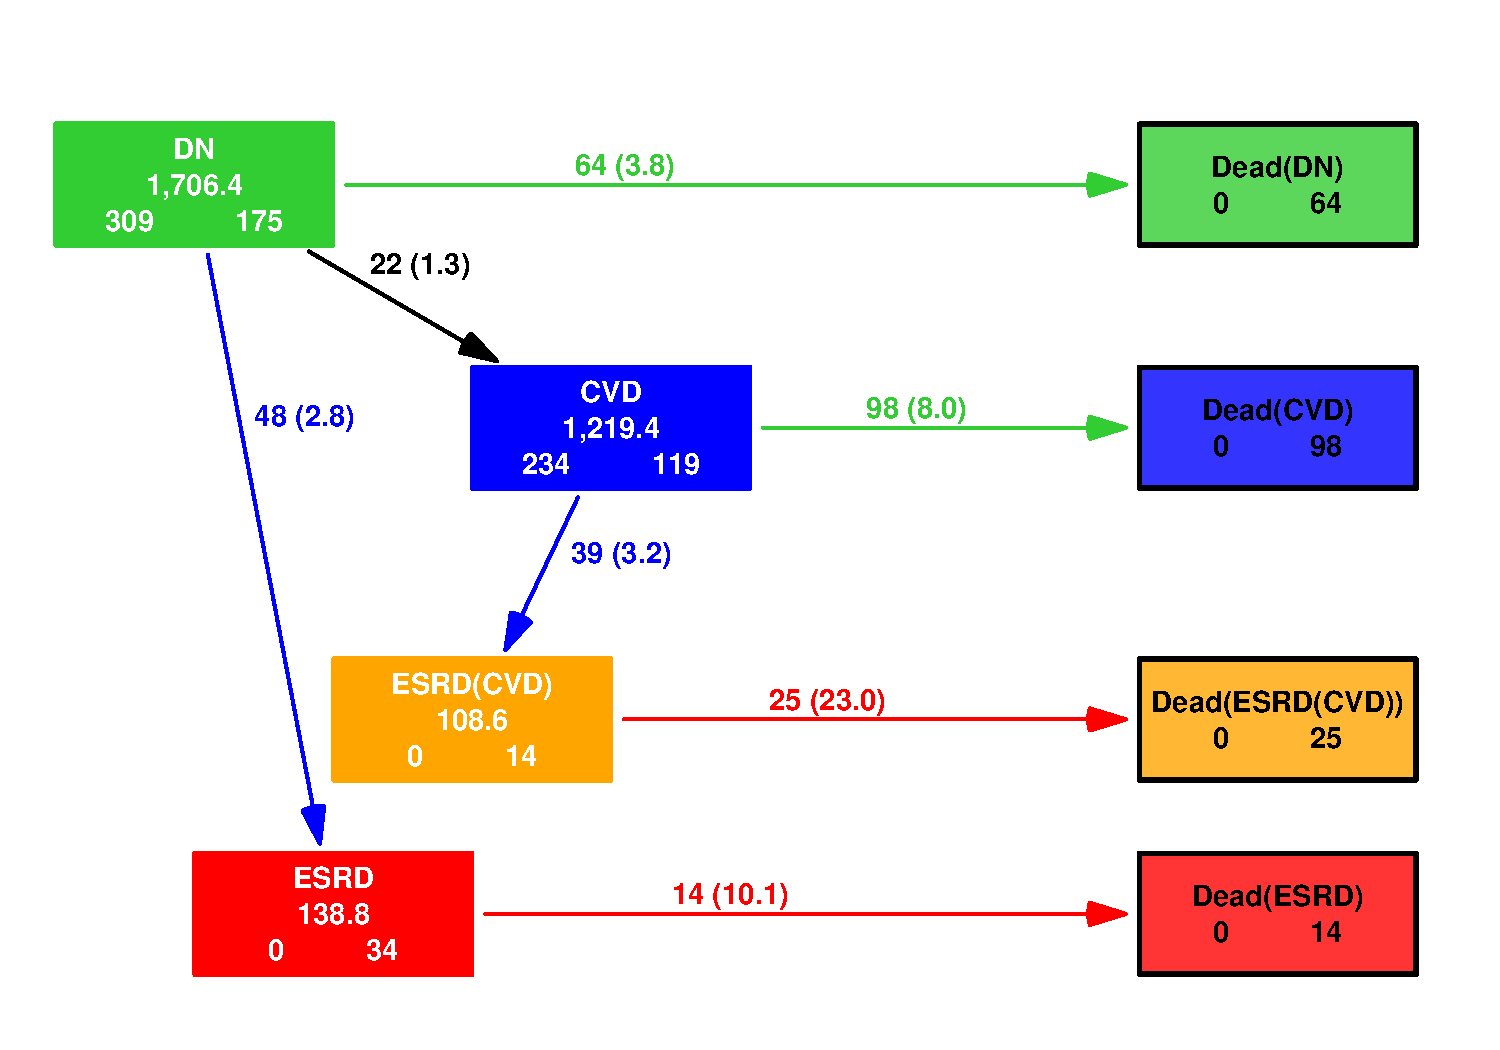
\includegraphics[width=0.45\textwidth]{./GbAd-states.pdf}
\vspace*{-1ex}
\renewcommand{\baselinestretch}{0.8}
\small
\begin{semiverbatim}
Tr <- list( "DN" = list( "Dead(DN)"  = \alert<2>{E1d},
                         "CVD"       = \alert<3>{E1c},
                         "ESRD"      = \alert<4>{E1e} ),
           "CVD" = list( "Dead(CVD)" = \alert<2>{E1d},
                         "ESRD(CVD)" = \alert<4>{E1e} ),
          "ESRD" = list( "Dead(ESRD)"= \alert<5>{E1n} ),
     "ESRD(CVD)" = list( "Dead(ESRD(CVD))"= \alert<5>{E1n} ) )
\end{semiverbatim}
\normalsize
\renewcommand{\baselinestretch}{1.0}

\end{frame}

% %----------------------------------------------------------------------
% \begin{frame}[fragile]
%    \frametitle{Construction of the \texttt{glm}s}
% \renewcommand{\baselinestretch}{0.8}
% \small
% \begin{semiverbatim}
% E1d <- glm( \alert<2>{lex.Xst %in% c("Dead(DN)","Dead(CVD)")} ~
%                               Ns( age, kn=a.kn ) +
%                               Ns( dur, kn=d.kn ) +
%                               Ns( tfn, kn=n.kn ) +
%                               (...) +
%                               \alert<4>{I(lex.Cst=="CVD")},
%             offset = log(lex.dur),
%             family = poisson,
%    data = subset( S5, \alert<3>{lex.Cst %in% c("DN","CVD")} ) )

% E1c <- update( E1d, \alert<5>{(lex.Xst=="CVD")} ~ .,
%                     data = \alert<6>{subset( S5, lex.Cst=="DN" )} )
% \end{semiverbatim}
% \normalsize
% \renewcommand{\baselinestretch}{1.0}
% \vspace*{-1ex} \hfill
% 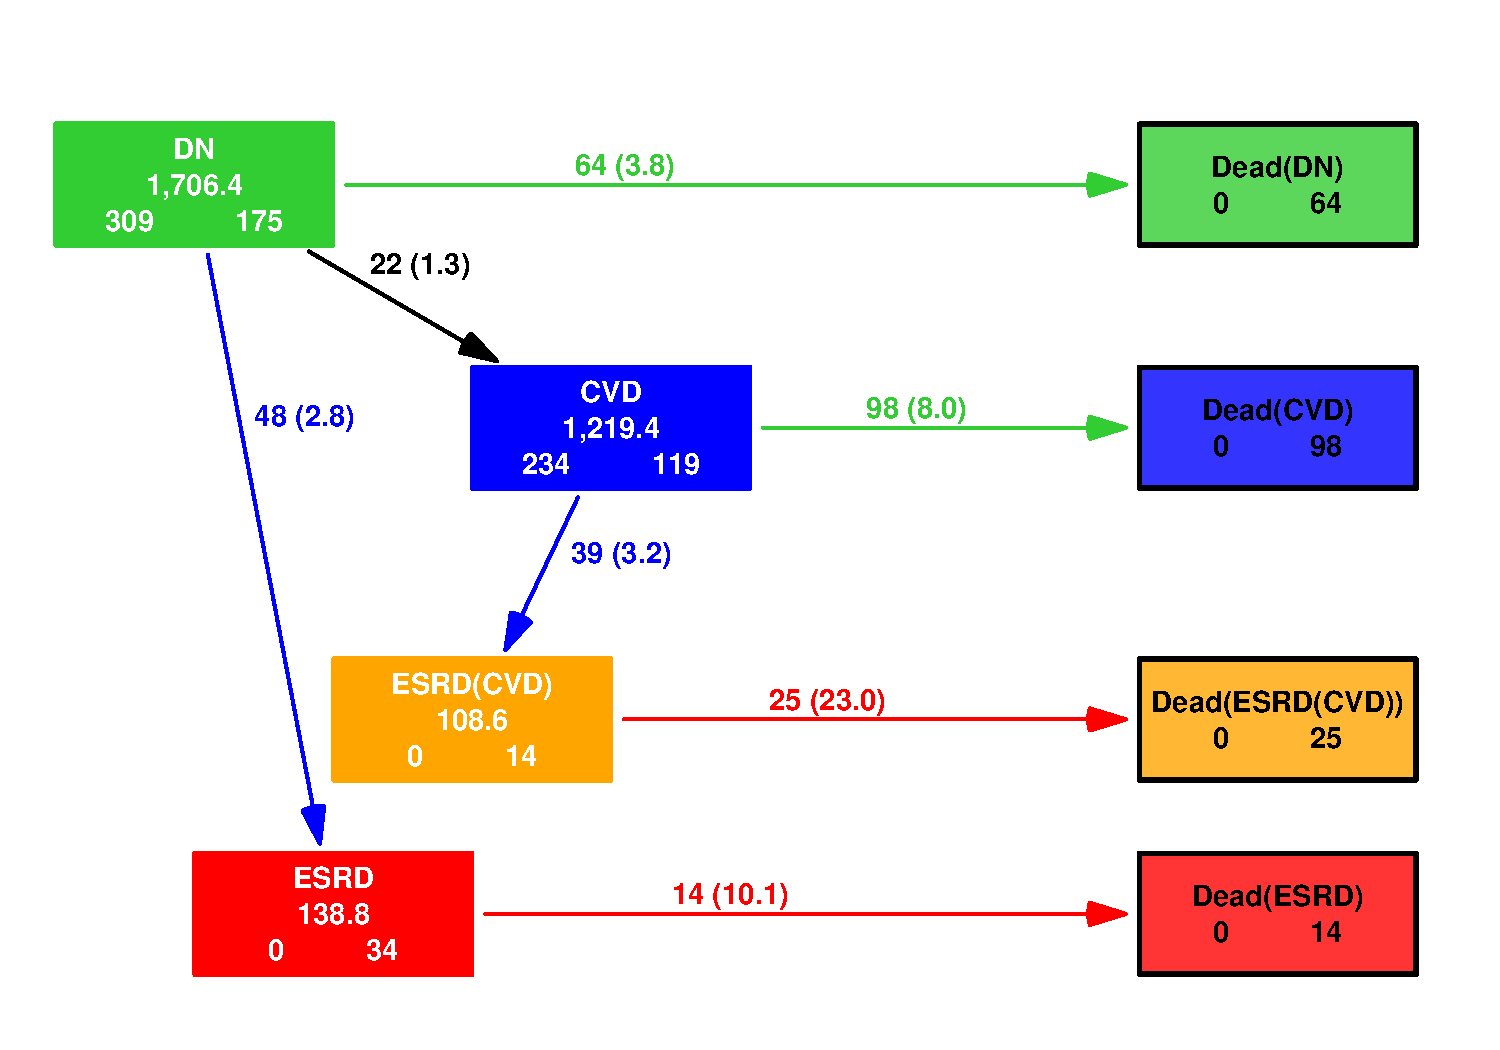
\includegraphics[width=0.3\textwidth]{./GbAd-states.pdf}
% \end{frame}

% \end{document}

%----------------------------------------------------------------------
\begin{frame}
   \frametitle{\texttt{simLexis}}
Input required:
   \begin{itemize}[<+->]
   \item A \texttt{Lexis} object representing the initial state of the persons
     to be simulated.\\
   (\texttt{lex.dur} and \texttt{lex.Xst} will be ignored.)
 \item A transition object with the estimated Poisson models collected
   in a list of lists.
   \end{itemize}

\pause
Output produced:
\pause
\begin{itemize}[<+->]
\item A \texttt{Lexis} object with simulated event histories for may persons
\item Use \texttt{nState} to count how many persons in each state at
  different times
\end{itemize}

\end{frame}

%----------------------------------------------------------------------
\begin{frame}[fragile]{Using \texttt{simLexis}}
Put one record a new \texttt{Lexis} object (\texttt{init}, say).
representing a person with the desired covariates.

Must have same structure as the one used for estimation:\\[-1ex]

\renewcommand{\baselinestretch}{0.8}
\footnotesize
\begin{semiverbatim}
init <- subset( S5, \alert<2>{FALSE},
                    \alert<3>{select=}c(timeScales(S5),"lex.Cst",
                         "dm.type","sex","hba1c",
                         "sys.bt","tchol","alb",
                         "smoke","bmi","gfr","hmgb",
                         "ins.kg") )
init[\alert<4>{1},"sex"] <- "M"
init[\alert<4>{1},"age"] <- 60
...

sim1 <- simLexis( Tr1, init,
                  time.pts=seq(0,25,0.2),
                  N=500 ) )
\end{semiverbatim}
\normalsize
\renewcommand{\baselinestretch}{1.0}
\end{frame}

%----------------------------------------------------------------------
\begin{frame}[fragile]{Output from \texttt{simLexis}}
\renewcommand{\baselinestretch}{0.8}
\footnotesize
\begin{semiverbatim}
> summary( sim1 )

Transitions:
     To
From         DN CVD ES(CVD)   ES Dead(CVD) Dead(ES(CVD)) Dead(ES) Dead(DN)
  DN        212  81       0  145         0             0        0       62
  CVD         0  50       7    0        24             0        0        0
  ESRD(CVD)   0   0       3    0         0             4        0        0
  ESRD        0   0       0   70         0             0       75        0
  Sum       212 131      10  215        24             4       75       62

Transitions:
     To
From         Records:  Events: Risk time:  Persons:
  DN              500      288    9245.95       500
  CVD              81       31     667.90        81
  ESRD(CVD)         7        4      45.72         7
  ESRD            145       75     891.11       145
  Sum             733      398   10850.67       500
\end{semiverbatim}
\normalsize
\renewcommand{\baselinestretch}{1.0}
\end{frame}

%----------------------------------------------------------------------
\begin{frame}[fragile]{Using a simulated \texttt{Lexis} object --- \texttt{pState}}
\renewcommand{\baselinestretch}{0.8}
\footnotesize
\begin{semiverbatim}
nw1 <- pState( nState( sim1,
                       at = seq(0,15,0.1),
                       from = 60,
                       time.scale = "age" ),
               perm = c(1:4,7:5,8) ) )
head( pState )
when       DN    CVD ES(CVD)     ES Dead(ES) Dead(ES(CVD)) Dead(CVD) Dead(DN)
  60   1.0000 1.0000  1.0000 1.0000   1.0000        1.0000    1.0000        1
  60.1 0.9983 0.9986  0.9986 0.9997   0.9997        0.9997    0.9997        1
  60.2 0.9954 0.9964  0.9964 0.9990   0.9990        0.9990    0.9990        1
  60.3 0.9933 0.9947  0.9947 0.9981   0.9981        0.9981    0.9982        1
  60.4 0.9912 0.9929  0.9929 0.9973   0.9973        0.9973    0.9974        1
  60.5 0.9894 0.9913  0.9913 0.9964   0.9964        0.9964    0.9965        1

plot( pState )
\end{semiverbatim}
\normalsize
\renewcommand{\baselinestretch}{1.0}
\end{frame}

%----------------------------------------------------------------------
\begin{frame}
   \frametitle{Simulated probabilities}
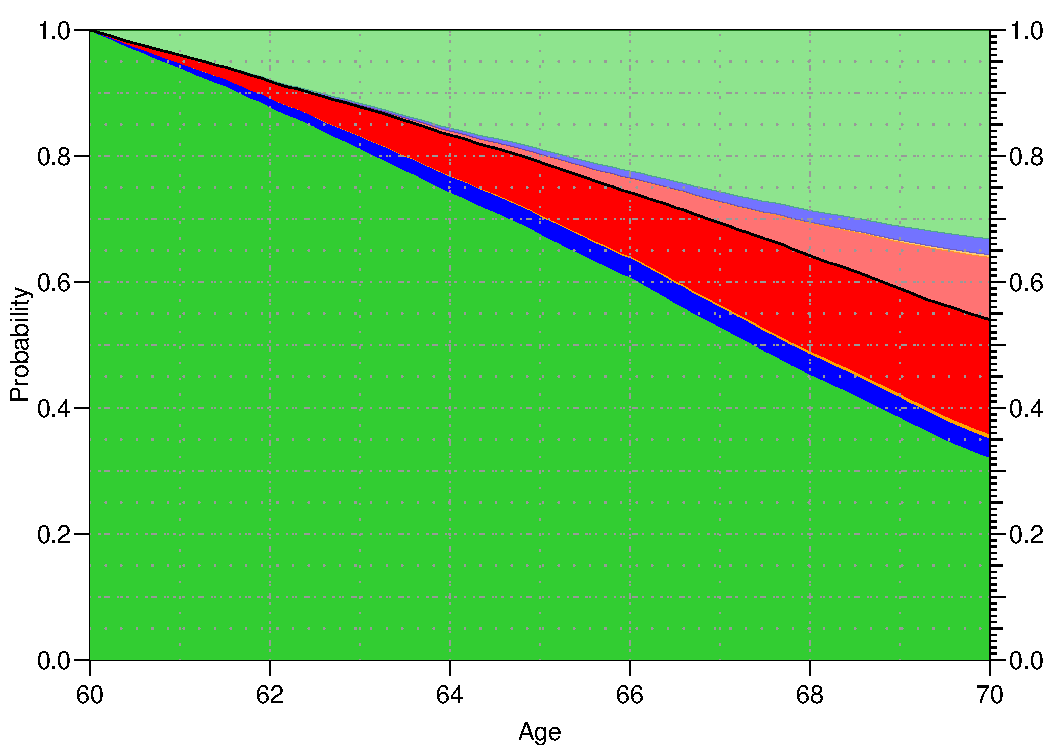
\includegraphics[width=0.75\textwidth]{./GbAd-probs.pdf}
\end{frame}

%----------------------------------------------------------------------
\begin{frame}
   \frametitle{How many persons should you simulate?}
\pause
   \begin{itemize}[<+->]
   \item All probabilities have the same denominator --- the initial
     number of persons in the simulation, $N$, say.
   \item Thus, any probability will be of the form $p=x/N$
   \item For small probabilities we have that:
\[
 \se\bigl(\log(\hat p)\bigr) = (1-p)/\sqrt{N p (1-p)}
\]
\item So c.i. of the form $p\td \erf$ where:
\[
 \erf = \exp\bigl( 1.96 \times (1-p)/\sqrt{N p (1-p)} \bigr)
\]
   \end{itemize}
\end{frame}

%----------------------------------------------------------------------
\begin{frame}
   \frametitle{Precision of simulated probabilities}
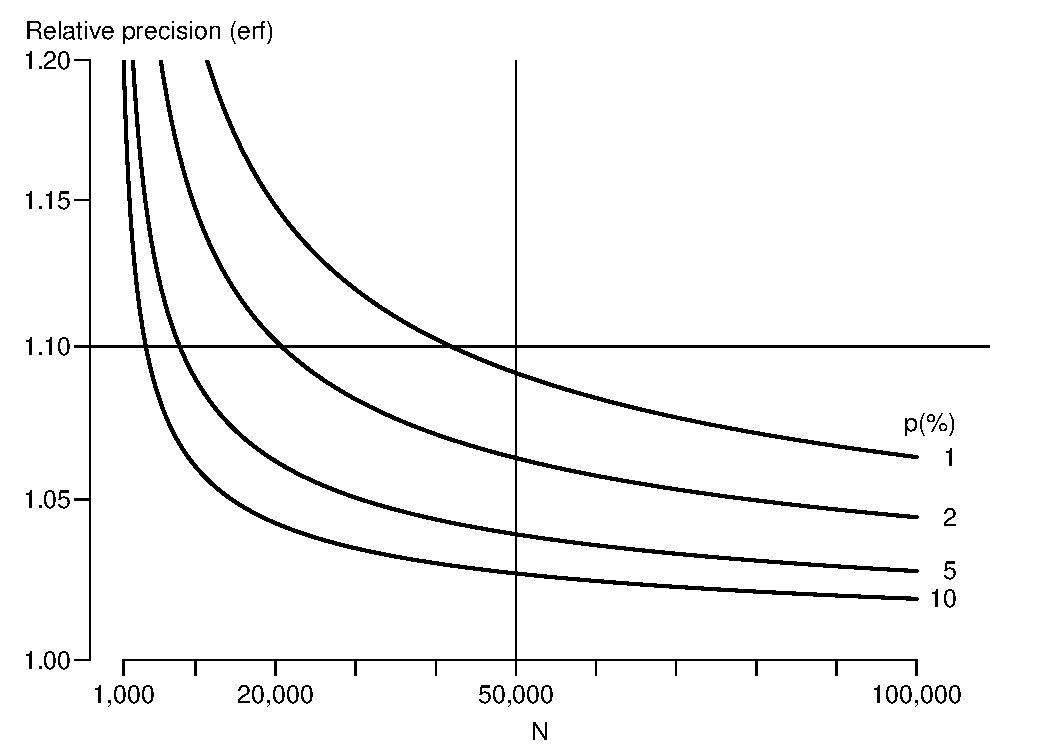
\includegraphics[width=0.75\textwidth]{./se-probs.pdf}
\end{frame}

%----------------------------------------------------------------------
\begin{frame}
   \frametitle{Multistate model overview}
\pause
   \begin{itemize}[<+->]
   \item Clarify what the relevant states are
   \item Allows proper estimation of transition rates
   \item --- and relationships between them
   \item Separate model for each transition (arrow)
   \item The usual survival methodology to compute probabilities breaks down
   \item Simulation allows estimation of cumulative probabilities:

     \begin{itemize}[<+->]
     \item Estimate transition rates (as usual)
     \item Simulate probabilities (\textbf{not} as usual)
     \end{itemize}

   \end{itemize}
\pause
Your turn: ``Renal complications''
\end{frame}

\end{document}
